\chap{Team Work}

\section{Agile implementation}
\vspace{-5mm}
As mentioned, Agile is based around incremental iterations, and this project was \\developed throughout three iterations. During each iteration, the Agile development process described in section 2.1.2 has been followed in the best way possible, learning from errors and trying to improve the process from one iteration to the next.

\subsection{First iteration}
\vspace{-5mm}
We started off by deciding which direction we wanted to go; the aim of the application. It was also decided that the first iteration should be focused around the general structure of the platform: static pages (home, about, help, etc.) and basic functionality. \\\\
During the second group meeting we made sketches of the different pages and how we wanted them to look, behave and interact with each other. Also, we planned the basic structure of the schema for the models (see Figure \ref{fig: Models}).\\\\
After design the basic structure, we created several user stories for this iteration, and stored them in a shared document, via Google Drive. Some examples of the stories are:
\vspace{-5mm}
\begin{itemize} \setlength{\itemsep}{-5pt}
\item As a public user, I'll be able to reach the home page. 1 point
\item As a public user, I'll need to be able to create a private user. 5 points
\item As an admin, I'll be able to see the list of users. 5 points
\end{itemize}
\pagebreak
This iteration was the most difficult one, code-wise, due to the relatively steep learning curve of Ruby on Rails. None of us had any prior experience with this framework. For the first few weeks we learned a tremendous amount about Ruby on Rails by reading, and coding along with the very extensive tutorial by Michael Hartl\cite{hartl}.\\\\
It took some time to get used to the framework, and maby we were a bit too enthusiastic, so we ended the first iteration completing around 80\% of the planned user stories.

\subsection{Second iteration}
\vspace{-5mm}
With the basic structure of the application implemented, we planned the second iteration with a bit more modesty than the first. This time, we tried to be more effective and organized and started to use \textit{Pivotal Tracker}\cite{pivotal} for user stories. The improvement of using this platform instead of Google Drive is explained in Section \ref{Pivotal_Tracker}.\\\\
The goal of this iteration was to implement the complete functionality of the platform. We re-planned  the structure of the different web pages, introducing a more advanced functionality. For example, we decided to add timetable subscription to the user functionality.\\
Ruby offers a very easy use of foreign keys; the way one is able utilize the same variable throughout different models, is genius. Mixing HTML and Ruby is also an excellent way to make our lives a lot easier.\\
Even though we weren't able to implement all the user stories scheduled, we did almost everything and had to re-plan just a few things for the third and last iteration. In order to plan it properly, we made a document listing all the errors and bugs we stumbled upon during the two first iterations..

\subsection{Third iteration}
\vspace{-5mm}
The work planned for this one was separated in three parts: 
\vspace{-5mm}
\begin{itemize}\setlength{\itemsep}{-5pt}
	\item[1.] Finish the leftover work from iteration two.
	\item[2.] Improve the graphical interface of the website.
	\item[3.] Sorting out bugs.
\end{itemize}
During this iteration, we did "small" agile iterations, due to the fact we were fixing problems and reiterating the code. \\
We finished the iteration with a fully functioning version of the application, and all the planned functionality implemented.
	
\section{Team cooperation and communication}
\vspace{-5mm}
Promote cooperation and communication between team members is probably one of the most important thing during a group project development process. Most of the time it's hard to figure out a good way for cooperate and communicate between each other, and also during this project it has been an relative issue, in particular in the first part of the project. It was mainly caused by different schedules, lectures and available time of each member of the team.
Even that, every single team member agreed about the importance of frequent meetings, so we almost always planned a group meeting once per week. 
The main communication way between the team member has been a chat group: it was used for decide team meeting and also to update the other teams about ideas or news about the code.
We basically spent the meeting's time:
\vspace{-5mm}
\begin{itemize}
 \setlength{\itemsep}{-5pt}
 \item Helping each other with any kind of problems about the project.
 \item Discussing new ideas.
 \item Planning what to do in the following period.
\end{itemize} 
\vspace{-5mm}

\section{Instruments and Applications usage}
\vspace{-5mm}
	\subsection{Git}
	\vspace{-5mm}
During the whole project development \textbf{Git} has been an indispensable instrument.\\
It is possible to define Git as a version control system, which means that the principal purpose is to help a software team manage changes to source code over time. In particular, it keeps track of every modification to the code in a special kind of database and, if a mistake is made, developers have the possibility to turn back and compare earlier version of the code in order to fix the mistake.\cite{versionController}\\
During this project, Git usage has been improved a lot between the first iteration and the last one. For example, during the first part of the project there were several problems about merging and push/pull of code, mainly caused by a lack of knowledge about how to use this system in a proper way. Then, once learnt from our mistakes, during the following parts of the project Git usage has been improved a lot and it provided a significant help to the team work. Probably the most appreciated Git function during this project was the possibility to always check out the latest version of the code, since all the team members were committing code quite often.

	\subsection{Pivotal Tracker} \label{Pivotal_Tracker}
	\vspace{-5mm}
As we have explained before, we did user stories in a shared document in the first iteration; it resulted not very productive. Thus, we looked for some tool to improve the usefulness of user stories. We found \href{https://www.pivotaltracker.com/}{Pivotal Tracker}, a website that let you start a project and add user stories to it. They have the format before explained (see Section \ref{Agile}), and also let you give each story Fibonacci points. Furthermore, it let you add different tasks to each story, which makes very easy to schedule your work and to see others' progress. Also, a person can "choose" a task, and marked it as \textit{started}, thus others would know which tasks have already a "owner".
\begin{figure}[H]
	\centering
	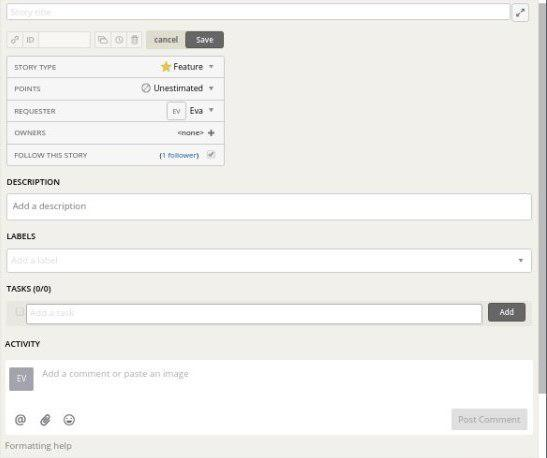
\includegraphics[trim={0 0 0 0},clip,width=1\textwidth]{Files/user_story.jpg}
	\caption{User Story from Pivotal Tracker}
	\label{fig: MVC}
\end{figure}

